
We report two sets of results. First, we examine the \emph{automation} mode, where each model solves the task directly. It is imperative to acknowledge here that these results characterize models' performance on single-turn, bounded professional deliverables completed \emph{without} tool usages. This setting differs from public agentic benchmarks, which often evaluate multi-step tool use, planning, and interaction with external environments; model orderings from those benchmarks therefore need not transfer to the setting studied here.

Second, we examine the \emph{augmentation} mode, where each assistant model acts as a coach that supplies a process guidance to a fixed GPT-3.5-Turbo worker that produces the final output, rather than solving the task itself. We then compare augmentation rankings to automation rankings to test whether strong direct task-solving ability also implies strong assistant ability. Across both analyses, rankings are computed over ten independent runs of the full pipeline. Main-text figures report within-task \emph{rank of ranks} (integer ranks derived from mean ranks across runs); the supplementary document reports mean rank with standard error ($\mathrm{SE}=\mathrm{SD}/\sqrt{10}$). All rankings are computed over the full candidate pool, which includes the unaided GPT-3.5-Turbo baseline. The accompanying supplementary materials provide the detailed audit trail for readers who wish to inspect individual tasks, models, and judgments.

Our central result is that model performance is both task-specific and mode-specific. In automation, rankings are concentrated around a small set of strong direct solvers, although this ordering should be interpreted as specific to
the bounded, single-turn tasks evaluated here rather than as a universal ranking of model capability. In augmentation, no single assistant model dominates across all tasks: different task domains reward different assistant behaviors, and several tasks are best handled by the unaided worker baseline rather than by an external assistance. This divergence suggests that standard automation benchmarks do not capture an economically important capability, whether a model can improve another worker's output through planning and decomposition. We use the paper figures to summarize the main patterns; the interactive dashboard provides a more detailed audit trail for readers who wish to inspect individual tasks, models, and judgments.

\subsection{Model Rankings in Automation Mode}

\begin{figure}[htbp]
    \centering
    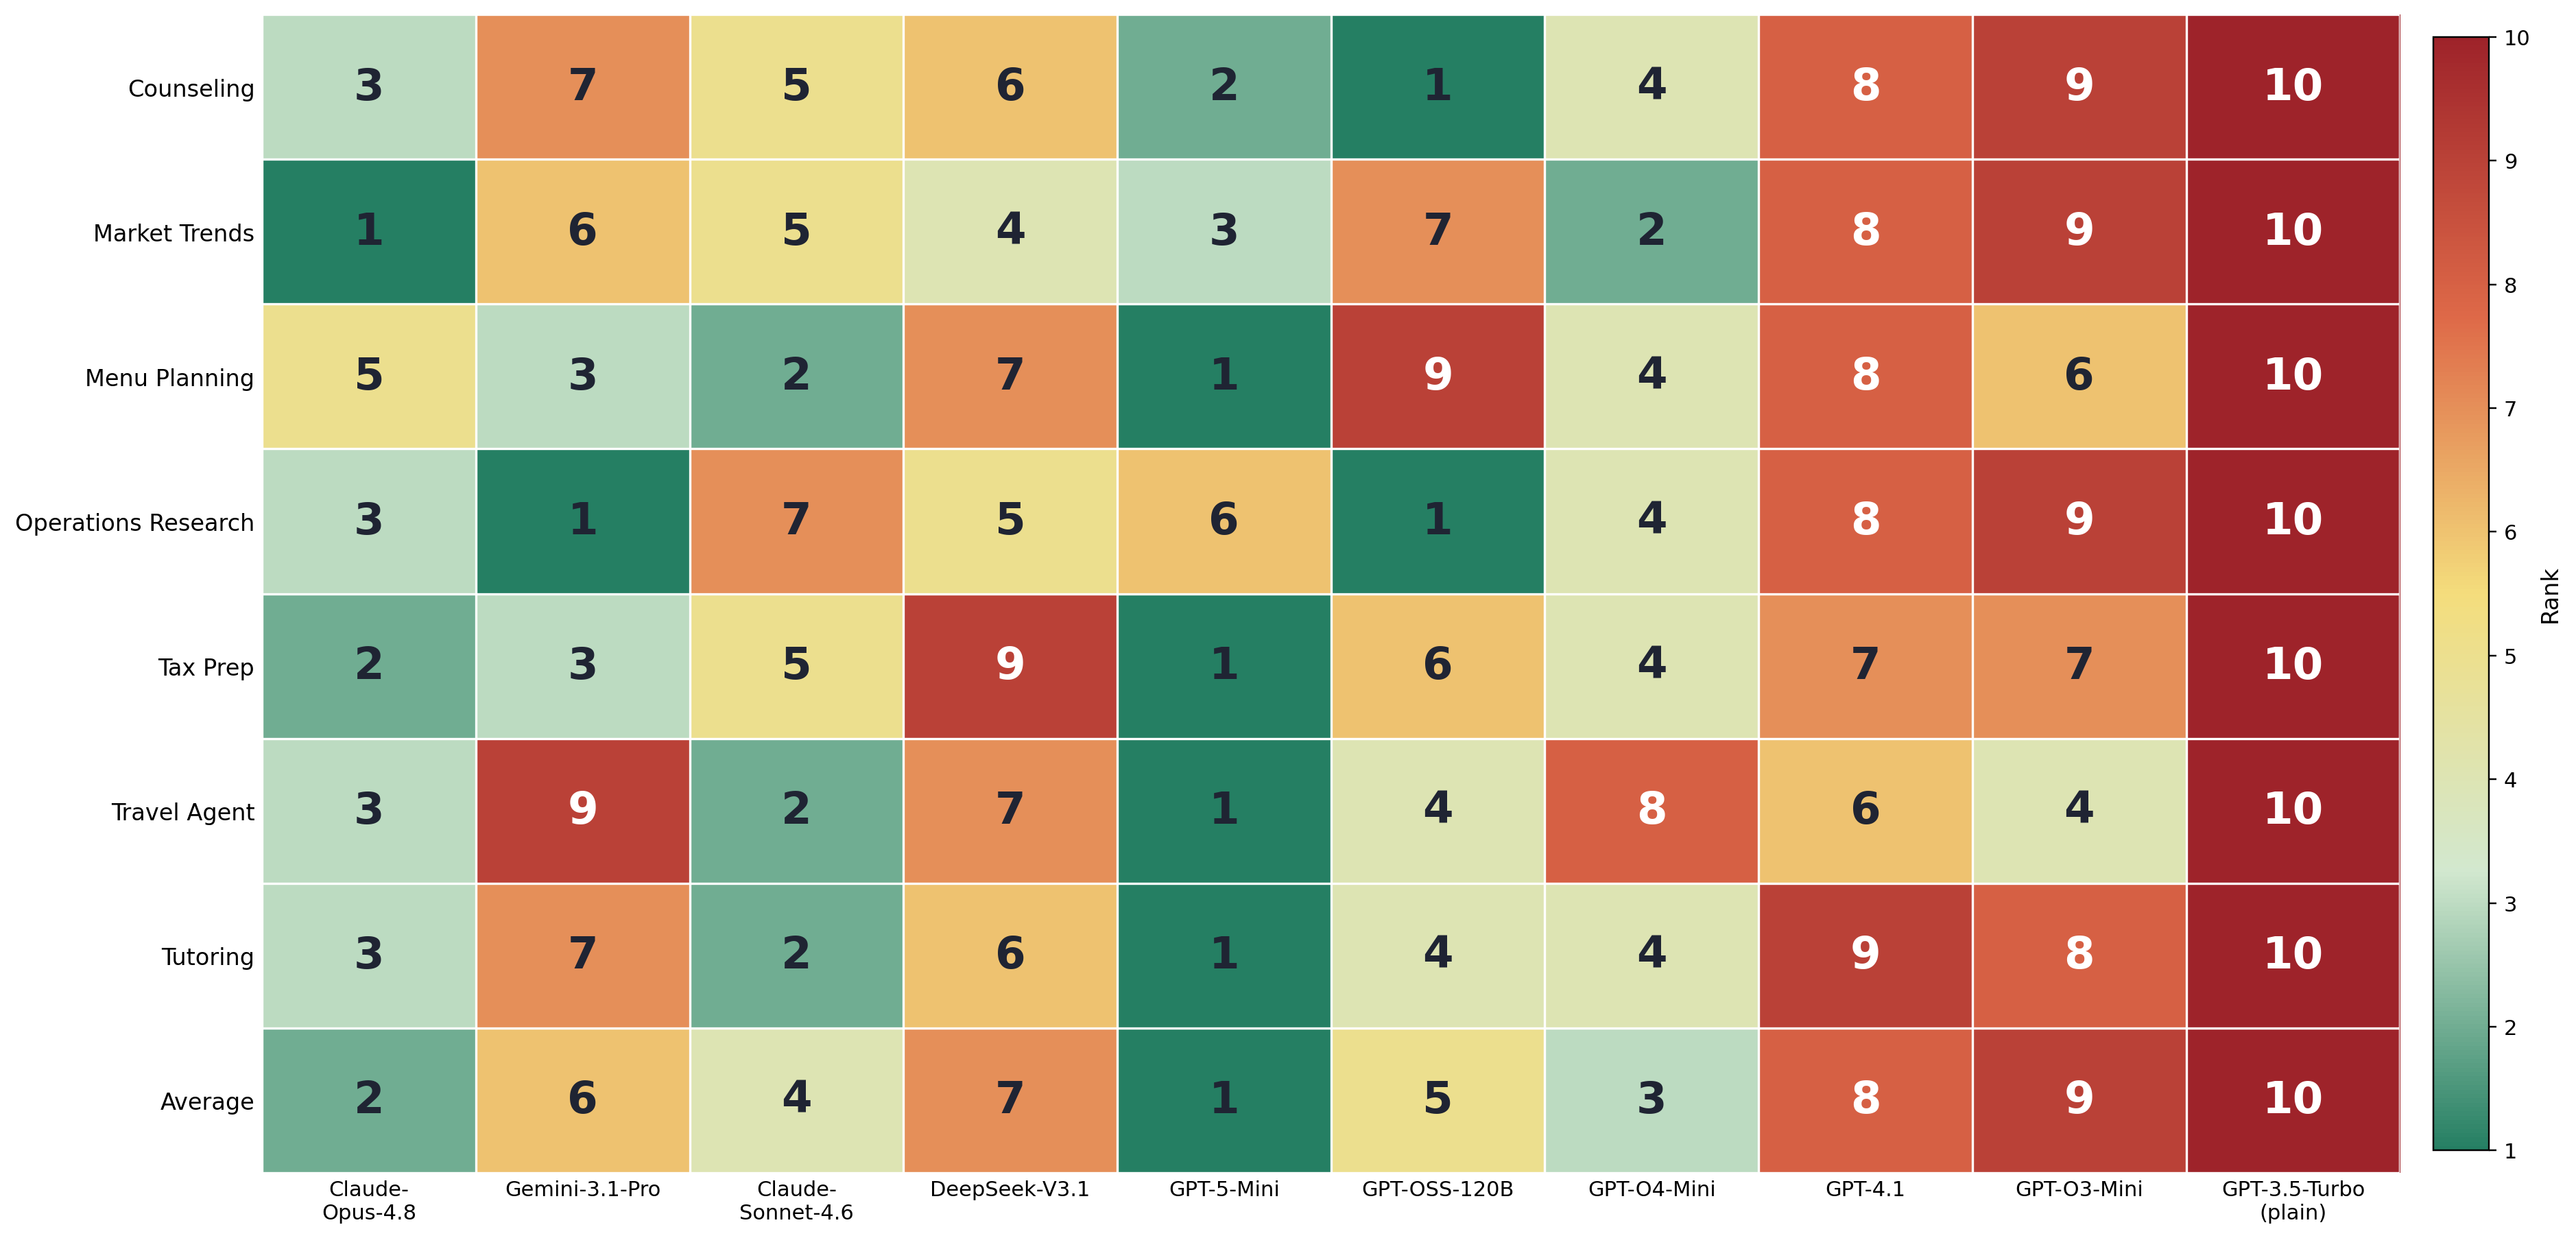
\includegraphics[width=\linewidth]{figures/figure2a_automation_heatmap.png}
    \caption{\textbf{Automation rankings by task, averaged across ten independent runs.} For each task, we first average each model's within-run rank across the ten runs and then rank these mean values to produce the displayed rank of ranks (1 = best). Rankings are computed using unrounded mean ranks. Exact ties receive the same rank, with the subsequent rank skipped (e.g., 1, 1, 3). Models are ordered from newest to oldest from left to right. Lower ranks indicate better performance. Mean ranks and standard errors are reported in the supplementary document.}
    \label{fig:automation-heatmap}
\end{figure}
% change model capability language
% In automation, rankings are directionally aligned with conventional capability rankings. Stronger frontier models tend to perform better as direct task solvers, while weaker or older models fall toward the bottom. Figure~\ref{fig:automation-heatmap} reports these rankings by task. GPT-5-Mini has the best average rank across tasks, followed by Claude-Opus-4.8. GPT-O4-Mini and Claude-Sonnet-4.6 form the next tier, while GPT-3.5-Turbo (plain) ranks last on average, as expected for a low-cost baseline. This is reassuring before we turn to augmentation, as stronger direct solvers are recognized as such across most task domains.

Figure~\ref{fig:automation-heatmap} reports model rankings in the automation mode by task across ten independent runs. GPT-5-Mini has the best average rank across tasks, followed by Claude-Opus-4.8. GPT-O4-Mini and Claude-Sonnet-4.6 form the next tier, while GPT-3.5-Turbo (plain) ranks last on average. The task-level results are also relatively concentrated. GPT-5-Mini ranks first in menu planning, tax preparation, travel planning, and tutoring; Claude-Opus-4.8 ranks first in market-trends analysis; GPT-OSS-120B ranks first in counseling; and GPT-OSS-120B and Gemini-3.1-Pro jointly lead operations research. 

The automation results characterize direct task performance under the particular roles, tasks, and interaction constraints studied here. Automation places the full burden of task completion on the model. It must interpret the prompt, track constraints, produce the final deliverable, and avoid errors without help from another system, so general model capability matters more. We next examine whether these same models retain their relative advantages when they instead assist a fixed downstream worker.
%The task-level pattern is also concentrated. GPT-5-Mini ranks first in menu planning, tax preparation, travel planning, and tutoring. Claude-Opus-4.8 ranks first in market-trends analysis, GPT-OSS-120B ranks first in counseling, along with Gemini-3.1-Pro jointly leading in operations research. A likely reason automation tracks conventional capability more closely is that it places the full burden of task completion on the  model. It must interpret the prompt, track constraints, produce the final deliverable, and avoid errors without help from another system, so general model capability matters more. Augmentation, by contrast, tests whether a model can improve a fixed worker's output through guidance; this depends not only on raw task-solving ability but on whether the guidance is usable by the worker. We examine that regime next.

\subsection{Model Rankings in Augmentation Mode}

\begin{figure}[htbp]
    \centering
    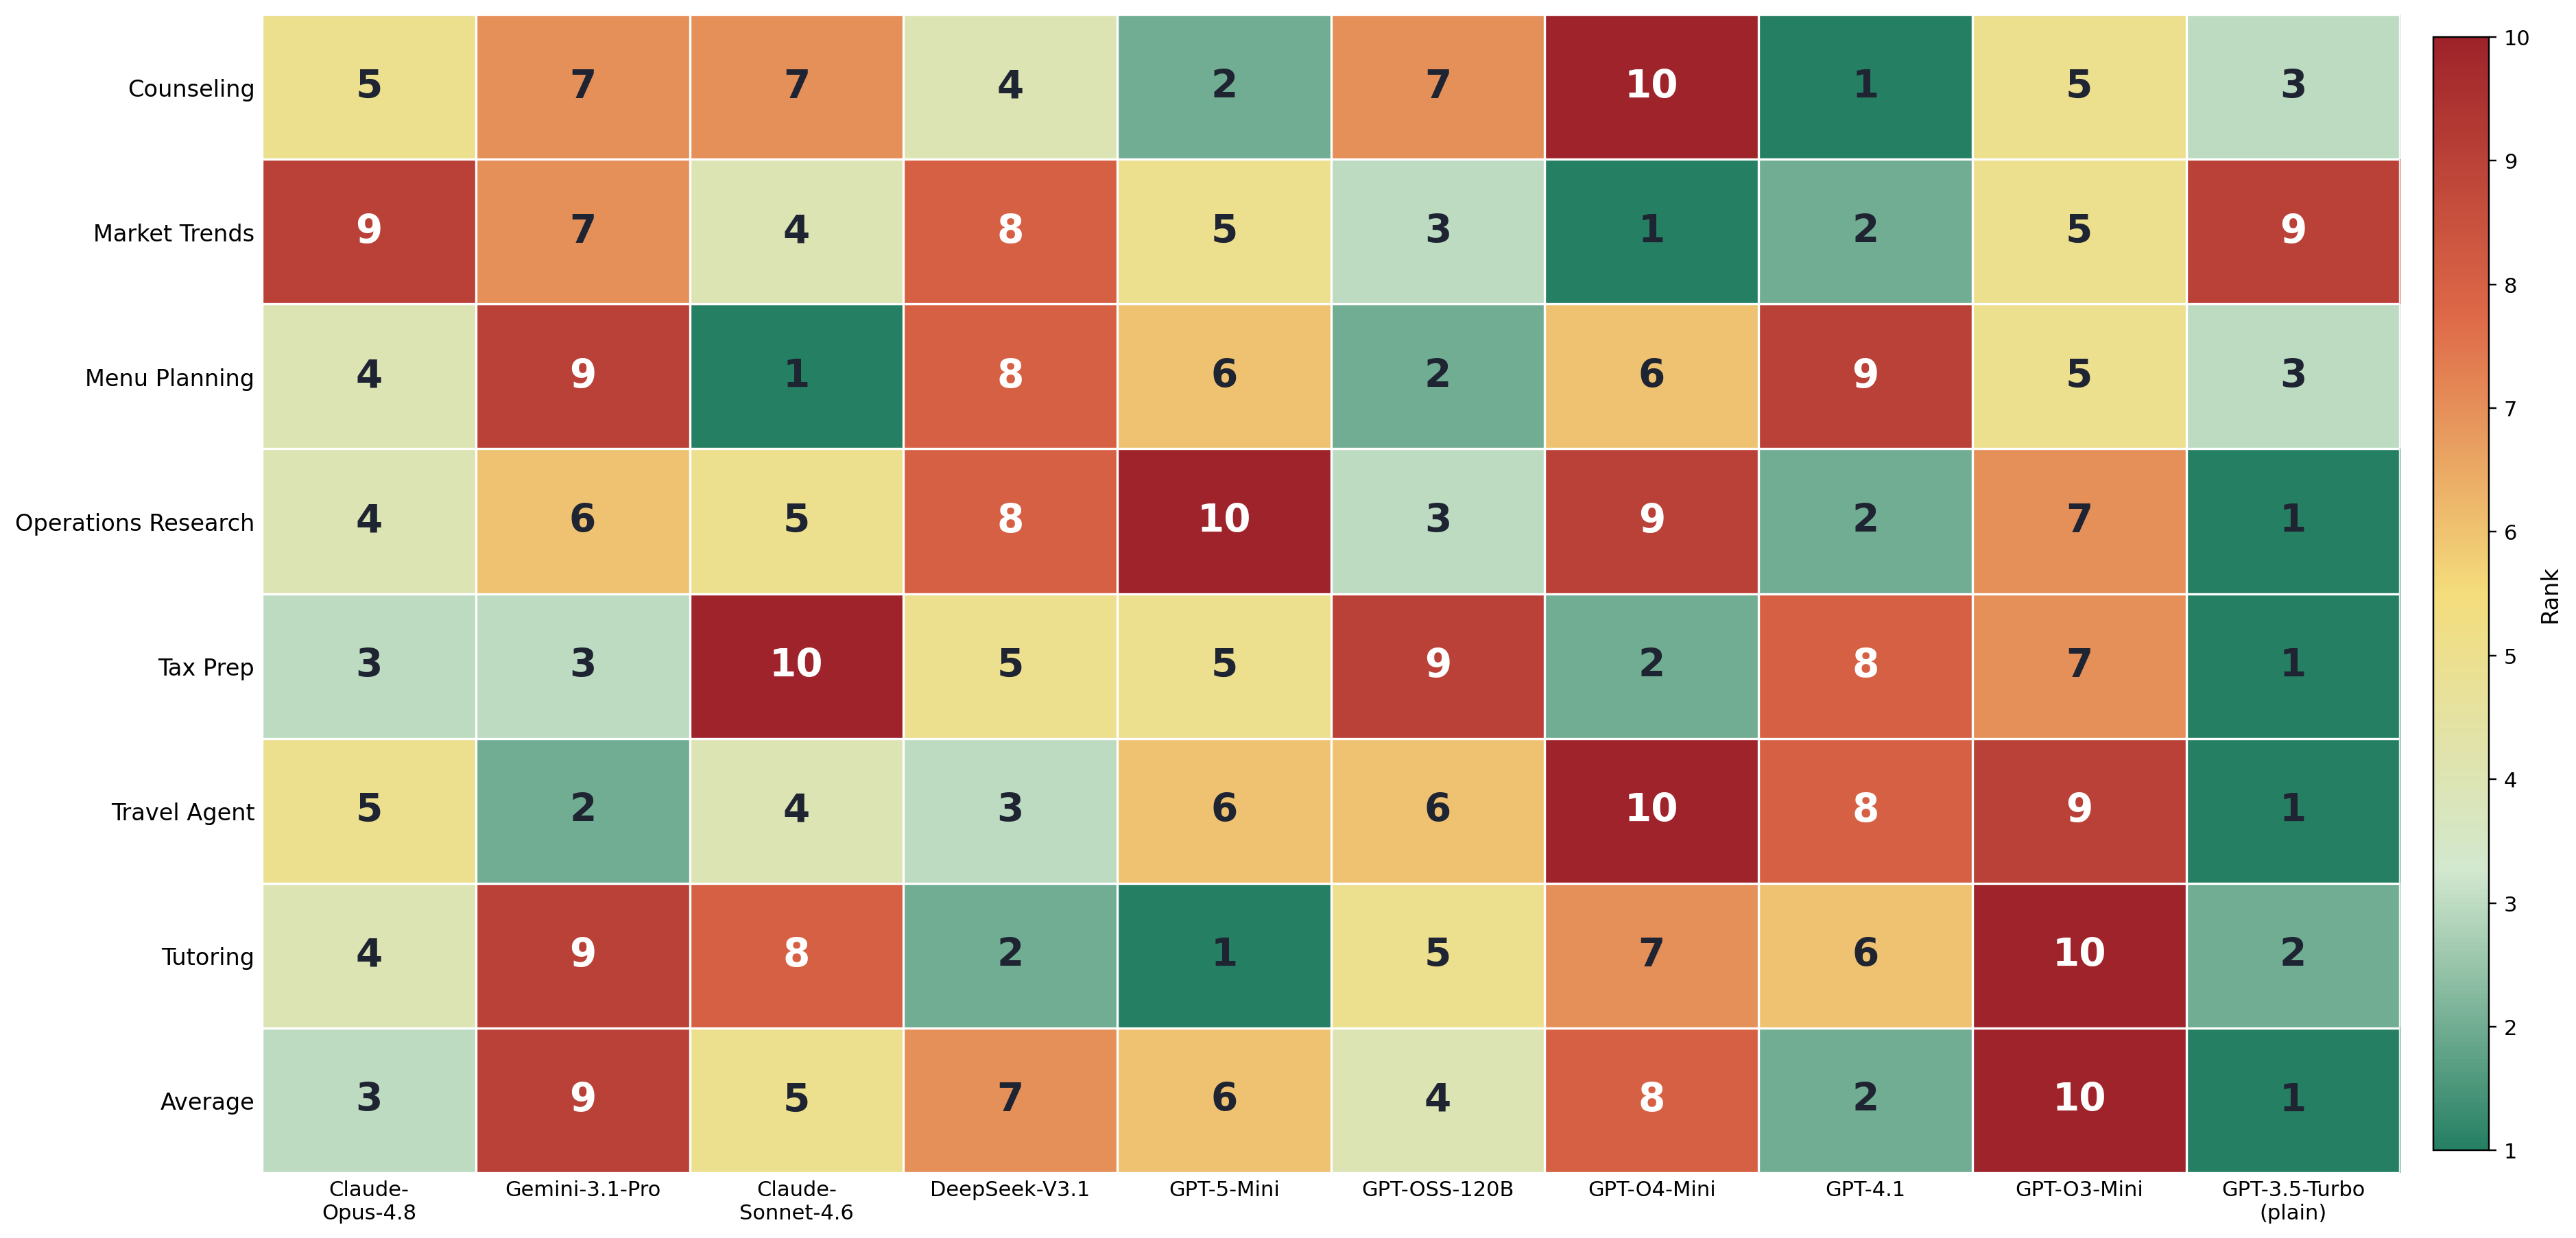
\includegraphics[width=\linewidth]{figures/figure1_augmentation_heatmap.png}
    \caption{\textbf{Augmentation rankings by task, averaged across ten independent runs.} For each task, we first average each model's within-run rank across the ten runs and then rank these mean values to produce the displayed rank of ranks (1 = best). Rankings are computed using unrounded mean ranks. Exact ties receive the same rank, with the subsequent rank skipped (e.g., 1, 1, 3). Models are ordered from newest to oldest from left to right, with GPT-3.5-Turbo (plain), the unaided worker baseline, shown at far right. Lower ranks indicate better performance. Mean ranks and standard errors are reported in the supplementary document.}
    \label{fig:augmentation-heatmap}
\end{figure}

Figure~\ref{fig:augmentation-heatmap} reports model rankings in the augmentation mode across ten independent runs. Each assistant model provides a process guidance in a form of an assistance text to a fixed GPT-3.5-Turbo worker, which then produces the final task output. The figure shows substantial heterogeneity across tasks: no single assistant model consistently ranks first across the task set, and the relative ordering of models shifts across counseling, tutoring, planning, and analytical tasks.

Unlike automation, the best assistant changes substantially across tasks in augmentation. GPT-4.1 ranks first in counseling, GPT-O4-Mini in market-trends analysis, GPT-5-Mini in menu planning and tutoring. However, the unaided GPT-3.5-Turbo worker baseline ranks first in operations research, tax preparation, and travel planning when it is included in the full candidate pool. The best-performing assistant therefore differs by domain rather than converging on a single model, and in some tasks assistant guidance does not improve on the fixed worker's unaided output, even worsening it.

The pattern also differs by task type. Among the assistant models, GPT-4.1 performs especially well in counseling, consistent with strength in professionally framed guidance and sensitive response structure. GPT-O4-Mini leads in market-trends analysis, where the rubric rewards concise synthesis, specificity, and actionable interpretation. GPT-5-Mini leads in menu planning and tutoring and is the best assistant in tax preparation, suggesting strength on tasks that require constraint tracking, complete deliverables, and structured explanation. GPT-OSS-120B leads among assistants in operations research, where the rubric rewards optimization framing and trade-off reasoning. Claude-Sonnet-4.6 leads among assistants in travel planning, where practical sequencing, budget awareness, and itinerary usability are central. These results suggest that different models provide different kinds of useful guidance, but the mechanisms require qualitative analysis of the guidance and the resulting worker outputs, which we return to in Section~\ref{sec:analysis}.

Importantly, these ranking differences are unlikely to be driven by models excelling on one general evaluation dimension but not another. Across the five general rubric dimensions (instruction following, accuracy and specificity, practical usefulness, organization and readability, and tone/audience fit), most models receive similar relative scores on each dimension rather than specializing on a single axis; the supplementary document reports the corresponding profiles. Augmentation rankings therefore reflect differences in overall assistant quality and task fit rather than artifacts of how the general rubric is weighted. Models do not win because they are disproportionately strong on, say, organization but weak on accuracy. The task-specific pairwise outcomes point to genuine differences in how each model guides the fixed worker.

\subsection{Automation Rankings Differ From Augmentation Rankings}
\label{sec:role-swap}

To quantify the relationship between the two usage modes, let
$r^{(k)}_{mts}$ denote the within-task rank of assistant model $m$ on task
$t$, in usage mode $s\in\{\mathrm{auto},\mathrm{aug}\}$, and independent run
$k\in\{1,\ldots,10\}$, where lower values indicate better performance. We
first average over runs,
\begin{equation}
    \bar r_{mts}=\frac{1}{10}\sum_{k=1}^{10}r^{(k)}_{mts}.
\end{equation}
For each task, we then compute
\begin{equation}
    \rho_t=\operatorname{corr}_{\mathrm{S}}
    \!\left(
      \{\bar r_{mt,\mathrm{auto}}\}_{m\in\mathcal{M}},
      \{\bar r_{mt,\mathrm{aug}}\}_{m\in\mathcal{M}}
    \right),
    \label{eq:task-mode-correlation}
\end{equation}
where $\operatorname{corr}_{\mathrm{S}}$ is Spearman's rank correlation and $\mathcal{M}$ contains the nine assistant models evaluated in both usage modes. The unaided worker is excluded because it has no corresponding assistant model in automation. For the model-level comparison, we additionally average
$\bar r_{mts}$ over the seven tasks before computing the same correlation in each usage mode. Because reverse rank is a monotonic transformation of rank, it produces the same Spearman correlations.

\begin{figure}[htbp]
    \centering
    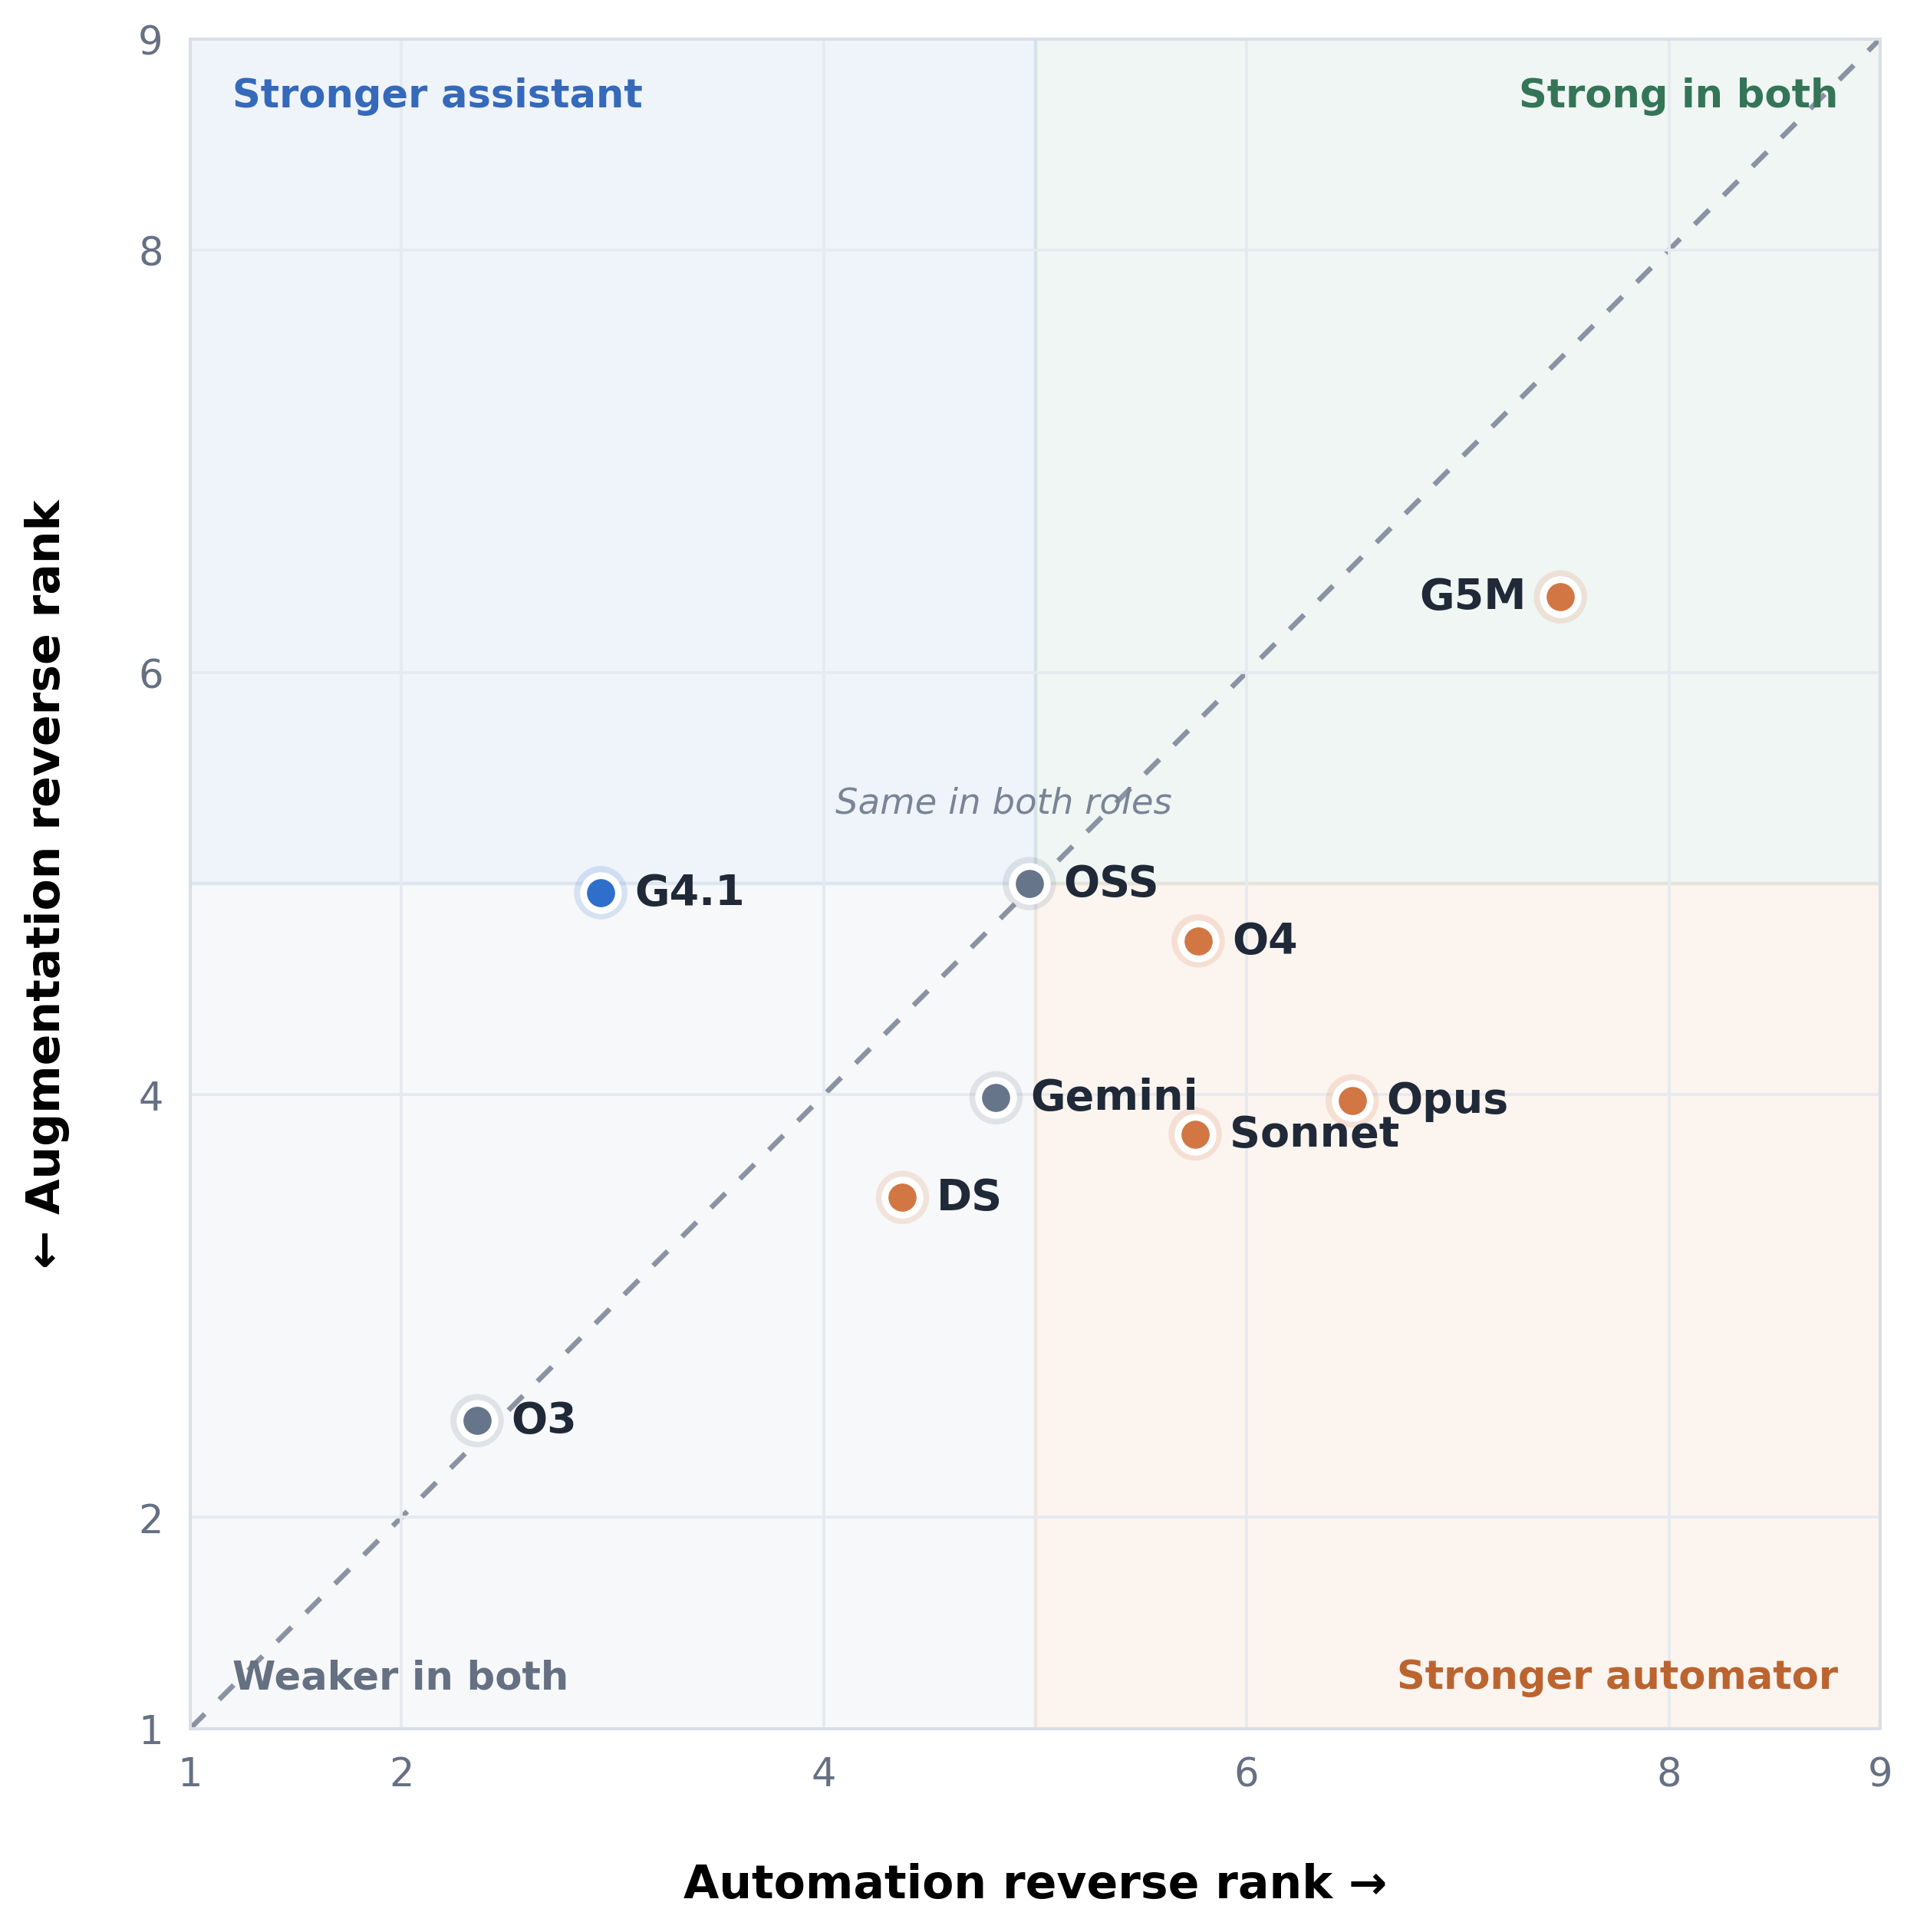
\includegraphics[width=0.79\linewidth]{figures/figure2b_role_swap_scatter_white.png}
    \caption{
    \textbf{Model-level comparison of average automation rank and average augmentation rank (assistant models only)}. 
    %Blue points report augmentation ranks and orange points report automation ranks; horizontal lines show the shift between regimes. Error bars show $\pm 1$ standard error, computed across ten independent runs after averaging ranks across tasks within each run. Lower rank indicates better performance.
    Each point represents one assistant model's average rank across seven tasks and ten independent runs. Ranks are inverted so that higher values indicate better performance. With nine assistant models, reverse rank is defined as \(10-\bar{r}\), where \(\bar{r}\) is the model's mean rank in the corresponding usage mode. The horizontal axis reports automation performance and the vertical axis reports augmentation performance. The unaided worker baseline is excluded.}
    \label{fig:role-swap-scatter}
\end{figure}

% Figure~\ref{fig:role-swap-scatter} compares each model's average automation rank and average augmentation rank. Several models move substantially across regimes. GPT-5-Mini is strong in both regimes and has the best average rank among assistant models in augmentation as well as the best average rank in automation. GPT-4.1 is relatively stronger as an assistant than as a direct solver: it ranks near the middle of the augmentation distribution but near the bottom in automation. Conversely, Claude-Opus-4.8, Claude-Sonnet-4.6, Gemini-3.1-Pro, and GPT-O4-Mini are stronger in automation than in augmentation. GPT-OSS-120B sits close to the diagonal, with similar average ranks across modes. The same model is thus not consistently favored when it solves a task directly versus when it assists another worker.

Figure~\ref{fig:role-swap-scatter} compares each model's average automation and augmentation rank. Across the nine shared assistant models, the Spearman rank correlation between automation and augmentation performance is moderate ($\rho=0.48$; two-sided $p=0.187$), but is not statistically distinguishable
from zero at conventional significance levels. GPT-5-Mini is strong in both usage modes and has the best average rank among assistant models in augmentation as well as the best average rank in automation. GPT-4.1 is relatively stronger as an assistant than as a direct solver. Conversely, Claude-Opus-4.8, Claude-Sonnet-4.6, Gemini-3.1-Pro, and GPT-O4-Mini are stronger in automation than in augmentation. GPT-OSS-120B sits close to the diagonal. Thus, automation performance contains some information about augmentation performance, but it is an incomplete proxy for it.


\begin{table}[htbp]
    \centering
    \small
    \begin{tabular}{lrr}
        \toprule
        Task & Spearman $\rho_t$ & $p$-value \\
        \midrule
        Tax Preparation & 0.85 & 0.004 \\
        Menu Planning & 0.64 & 0.066 \\
        Tutoring Session Planning & 0.50 & 0.166 \\
        Counseling & 0.25 & 0.516 \\
        Operations Research Analysis & 0.17 & 0.668 \\
        Market Trend Analysis & 0.10 & 0.798 \\
        Travel Planning & -0.04 & 0.915 \\
        \bottomrule
    \end{tabular}
    \caption{\textbf{Task-level correlation between automation and augmentation rankings.} Spearman correlations are computed across the nine assistant models using each model's mean rank over ten runs. Positive values indicate similar cross-mode ordering; values near zero indicate little correspondence. $p$-values are descriptive because each task contains only nine models.}
    \label{tab:mode-correlations}
\end{table}


The strength of this correlation varies substantially by task as shown by Table~\ref{tab:mode-correlations}. Tax preparation has the strongest cross-mode correlation ($\rho_{\mathrm{tax}}=0.85$), followed by menu planning ($\rho_{\mathrm{menu}}=0.64$) and tutoring ($\rho_{\mathrm{tutor}}=0.50$). The rankings are only weakly associated in counseling ($\rho=0.25$), operations research ($\rho=0.17$), and market trends analysis ($\rho=0.10$), and are essentially unrelated in travel planning ($\rho=-0.04$). Tax preparation is the only task whose association is statistically distinguishable from zero at the conventional level ($p=0.004$), including under a Bonferroni correction for seven task-level comparisons. Broader statistical significance across tasks would require a larger model pool or additional runs, and remains an avenue for future work.

The supplementary document's Table~\ref{tab:best-model-by-task} makes the divergence concrete. It reports the best-performing model in each task under automation and augmentation, using the lowest mean rank across ten runs. In five of seven tasks, the augmentation winner differs from the automation winner. In counseling, GPT-OSS-120B is the strongest automator while GPT-4.1 is the strongest assistant; in market-trends analysis, Claude-Opus-4.8 automates best but GPT-O4-Mini assists best; and in operations research, Gemini-3.1-Pro automates best while the unaided worker baseline ranks first in augmentation. Menu planning and tutoring are the two exceptions, where GPT-5-Mini ranks first in both usage modes.

The table also shows that augmentation winners are not uniformly frontier assistant models. GPT-3.5-Turbo (plain), the unaided worker with no external assistance, ranks first in operations research, tax preparation, and travel planning. Averaged across all seven tasks, the plain baseline has a mean rank
of $3.79$; GPT-5-Mini is the only assisted condition with a better overall mean rank of $3.66$. We read this not as evidence that guidance is futile, but as
evidence that its value is task-contingent and can be negative. Poorly matched or overly complex guidance can leave the worker worse off than working alone. The corollary is central to our argument that strong direct solvers do not automatically make strong assistants, and the right model depends jointly on the role it plays and the task it supports.

Lastly, several models exhibit large and reproducible
task-level role reversals. In market trends analysis, Claude-Opus-4.8 is the strongest automator (mean rank $2.05$) but one of the weakest assistants (mean rank $8.15$). Conversely, in counseling, GPT-4.1 ranks substantially better as an assistant (mean rank $3.80$, the best among assisted conditions) than as an automator (mean rank $7.40$). These differences persist after averaging across ten independent runs and therefore are not attributable to a single random run.

% seg into 4.4
The rankings establish that assistance quality is distinct from direct-solving ability, but they do not by themselves explain why particular assistance texts
help or hinder the downstream worker model. We therefore turn to the underlying assistance texts, worker outputs, rubric scores, and judge rationales. 
Section~\ref{sec:analysis} examines cases with especially large gaps between ranks to identify recurring differences between effective and ineffective assistance.

% The table also shows that augmentation winners are not uniformly frontier assistant models. GPT-3.5-Turbo (plain), the unaided worker with no external assistance, ranks first in operations research, tax preparation, and travel planning. We read this not as evidence that guidance is futile, but as evidence that its value is task-contingent and can be negative: poorly matched or overly complex guidance can leave the worker worse off than working alone. The corollary is central to our argument that strong direct solvers do not automatically make strong assistants, and the right model depends jointly on the role it plays and the task it supports. We interpret these qualitative differences in the guidance and final outputs in Section~\ref{sec:analysis}.

%% TODO - add a paragraph on correlations overall, and across tasks. (Done look above)

%% TODO - go back to the three results hihglighted in the intro and see that we covered all three (Checked)

%% TODO - we need an example for what is goiong on, either hre or start of next section

\subsection{Mechanisms: Preliminary Observations on Assistance Quality}
\label{sec:analysis}

To understand what traits make for effective augmentation, we turn to the education literature to ground our observational findings. \citet{wood1976}  coined the term ``scaffold'' to define the process that enables a learner to solve a task or achieve a goal that would be beyond their unassisted efforts. In their framing, as in ours, the expert guides the learner through a task rather than completing it for them. \citet{vandepol2010} take this concept further by identifying three essential properties of effective scaffolding: (1) contingency - support is calibrated to the learner's current level, (2) fading - support is gradually withdrawn as competence grows, and (3) transfer of responsibility - the goal is learner autonomy, not dependence. The first and third properties are most directly applicable to our single-interaction setting, where scaffolds cannot adapt over time. We apply this lens to our case in order to evaluate the LLM-generated assistance texts, which are analogous to the scaffolds in education. We compare the assistance texts received by the two highest-ranked outputs against those received by the two lowest-ranked outputs across all seven tasks. In doing so, we identify three characteristics of high-quality augmentation scaffolds.

%\begin{figure}[H]
\centering

\begin{minipage}[t]{0.485\textwidth}
\begin{tcolorbox}[
    enhanced,
    equal height group=or-assistance,
    colback=green!3,
    colframe=green!45!black,
    colbacktitle=green!45!black,
    coltitle=white,
    fonttitle=\bfseries\small,
    title={Higher-Ranked Assistance Text},
    boxrule=0.5pt,
    arc=2pt,
    left=6pt,
    right=6pt,
    top=5pt,
    bottom=5pt
]
\raggedright
\small
\textit{GPT-4.1, Operations Research, Run 2}

\medskip
\textbf{2.\ Plan and Structure}
\begin{itemize}
    \setlength{\itemsep}{3pt}
    \setlength{\parskip}{0pt}
    \item Outline a clear structure using logical headings aligned with each
    requirement.
    \item Allocate approximate word counts to each section to remain within
    the limit.
    \item Identify where to \textbf{highlight trade-offs and risk
    considerations in the recommendations}.
\end{itemize}

\textbf{3.\ Draft, Self-Review, and Finalize}
\begin{itemize}
    \setlength{\itemsep}{3pt}
    \setlength{\parskip}{0pt}
    \item \textbf{Ensure that all requirements are addressed and that the
    recommendations are balanced and well supported.}
\end{itemize}
\end{tcolorbox}
\end{minipage}
\hfill
\begin{minipage}[t]{0.485\textwidth}
\begin{tcolorbox}[
    enhanced,
    equal height group=or-assistance,
    colback=red!3,
    colframe=red!45!black,
    colbacktitle=red!45!black,
    coltitle=white,
    fonttitle=\bfseries\small,
    title={Lower-Ranked Assistance Text},
    boxrule=0.5pt,
    arc=2pt,
    left=6pt,
    right=6pt,
    top=5pt,
    bottom=5pt
]
\raggedright
\small
\textit{GPT-O3-Mini, Operations Research, Run 2}

\medskip
\textbf{2.\ Plan and Structure}
\begin{itemize}
    \setlength{\itemsep}{3pt}
    \setlength{\parskip}{0pt}
    \item Develop a high-level outline that organizes the content logically.
    \item Decide which headings could improve clarity.
    \item Integrate trade-offs and risks \textbf{without delving into specific
    solutions or analysis}.
\end{itemize}

\textbf{3.\ Draft, Self-Review, and Finalize}
\begin{itemize}
    \setlength{\itemsep}{3pt}
    \setlength{\parskip}{0pt}
    \item Finalize the document \textbf{without task-specific analytical
    content}.
\end{itemize}
\end{tcolorbox}
\end{minipage}

\caption{\textbf{Selected assistance-text excerpts for the operations research
task.} Intervening instructions are omitted for brevity. The higher-ranked
assistance text (left) directs the worker to address task requirements,
trade-offs, risks, and recommendations. The lower-ranked assistance text
(right) instead instructs the worker to avoid task-specific analysis, limiting
the usefulness of the resulting guidance.}
\label{fig:assistance-text-comparison}
\end{figure}

\begin{table}[htbp]
\centering
\definecolor{traitA}{RGB}{224,238,250} % soft blue
\definecolor{traitB}{RGB}{255,247,222} % soft yellow
\definecolor{traitC}{RGB}{250,228,228} % soft rose
\footnotesize
\setlength{\tabcolsep}{5pt}
\renewcommand{\arraystretch}{1.25}
\begin{tabularx}{\linewidth}{
    >{\raggedright\arraybackslash}p{1.0cm}
    >{\raggedright\arraybackslash}p{3.0cm}
    >{\raggedright\arraybackslash}X}
\toprule
 & \textbf{Task, assistant (rank)} & \textbf{Assistance-text excerpt} \\
\midrule

% run 4
\rowcolor{traitA} \multicolumn{3}{l}{\textbf{Trait 1: Specificity beyond the prompt (contingency)}} \\
\rowcolor{traitA} \textbf{Good} & Market trends, GPT-5-Mini (1) &
``For each trend, plan 2 to 3 succinct bullets: core observation, primary driver(s), and potential market implication\ldots a short preface about methodology and data vintage.'' \\
\rowcolor{traitA} \textbf{Bad} & Market trends, GPT-4.1 (9) &
``Ensure you understand the expectation to discuss how various factors (supply, demand, weather, storage, LNG exports, infrastructure, policy) interact\ldots'' \textit{(restates the prompt's factor list)} \\
\addlinespace

% run 1
\rowcolor{traitB} \multicolumn{3}{l}{\textbf{Trait 2: Explicit structure and ordering}} \\
\rowcolor{traitB} \textbf{Good} & Travel planning, Gemini-3.1-Pro (3) &
Enforces assumptions and clarifying questions ``\emph{before} the provisional itinerary,'' with named sections in explicit order: Introduction $\to$ Budget Breakdown $\to$ Daily Itinerary $\to$ Conclusion. \\
\rowcolor{traitB} \textbf{Bad} & Travel planning, GPT-O4-Mini (9) &
``Determine sequence and hierarchy of information for clarity and flow''; instructs worker to ``populate each section with neutral placeholders\ldots\ \emph{[Day 1: transportation placeholder]}''; no ordering is prescribed. \\
\addlinespace

% run 2
\rowcolor{traitC} \multicolumn{3}{l}{\textbf{Trait 3: Not working against the task}} \\
\rowcolor{traitC} \textbf{Good} & Operations research, Gemini-3.1-Pro (3) &
``Present two distinct, practical strategies. For each, explicitly state the expected benefits, potential drawbacks, and associated risks.'' \\
\rowcolor{traitC} \textbf{Bad} & Operations research, GPT-O3-Mini (9) &
``Establish a workflow for integrating\ldots trade-offs \textbf{without delving into specific solutions or analysis}''; finalize ``\textbf{without\ldots task-specific analytical content}.'' \\
\addlinespace

\bottomrule
\end{tabularx}
\caption{\textbf{Illustrative higher- vs.\ lower-ranked assistance texts for each
scaffold-quality characteristic.} Rows are color-coded by trait; ranks are the aggregate
augmentation rank within the task run. Excerpts are drawn from the assistance texts and lightly trimmed.}
\label{tab:trait-examples}
\end{table}


First, good guidance includes specificity that adds analytical value beyond the prompt, rather than just regurgitating information from the prompt, which is an application of the contingency principle, where effective scaffolding is calibrated to the learner's specific challenge rather than offered generically \citep{vandepol2010}. Table~\ref{tab:trait-examples} illustrates each trait with a higher- and lower-ranked assistance text. Low-performing guidance messages that simply echo the prompt's own constraints do not augment the focal worker, who already have access to the prompt. For example, in the market trends task, a top assistance text directs the worker to pair each trend with its primary driver and likely market implication and to note the underlying methodology, whereas a bottom-tier assistance text merely restates the prompt's own list of factors without adding an analytical step.

Next, embedding explicit structural requirements into the workflow is another trait of a top assistance text. In the travel planning task, a top assistance text enforces assumptions and clarifying questions before the provisional itinerary and prescribes a named section sequence (introduction, budget breakdown, day-by-day itinerary, and conclusion), making the ordering non-negotiable. A bottom-tier assistance text, by contrast, delegates ordering to the worker by instructing it to ``determine sequence and hierarchy of information for clarity and flow,'' and substitutes neutral placeholders for actual structural guidance.

Third, a negative point that good scaffolds avoid: actively working against task completion. Effective scaffolding includes what \citet{wood1976} term \textit{direction maintenance}, keeping the learner oriented toward the task objective. The most harmful assistance texts in our study invert this function entirely: rather than correcting learner drift, the scaffold itself redirects the worker away from the core deliverable, by instructing the worker not to finish the task as described in the prompt. In operations research task, a bottom ranked scaffold instructs the worker to establish a workflow for integrating necessary performance indicators, risk discussions, and balanced trade-offs without delving into specific solutions or analysis, yet the task explicitly requires two practical solutions with trade-offs stated. This instruction directly prohibits the core deliverable. Thus, no assistance can often beat bad assistance. Notably, the unaided worker is a strong baseline: the plain condition (GPT-3.5-Turbo with no assistance) ranks at or near the top in the many tasks. Poorly calibrated assistance is therefore frequently worse than none, undermining the transfer of responsibility that effective scaffolding aims to achieve \citep{vandepol2010}.

% OLD
%For tasks that require domain knowledge, such as tax law, a heavy assistant text that introduces caveating language or irrelevant processes can push the worker below its unassisted baseline. In fact, the plain condition (no assistance) tops the rankings for tax preparation. Extraneous advice, such as noting that gaps may prevent exact liability calculations, can be distracting or suggest hedging behavior, rather than letting the worker apply its own tax knowledge. This type of augmentation undermines the transfer of responsibility that effective scaffolding aims to achieve \citep{vandepol2010}.
